\subsection{Gaussians are bad for ICA}

\mode<presentation>{
\begin{frame} 
    \begin{center} \huge
        \subsecname
    \end{center}
    \begin{center}
    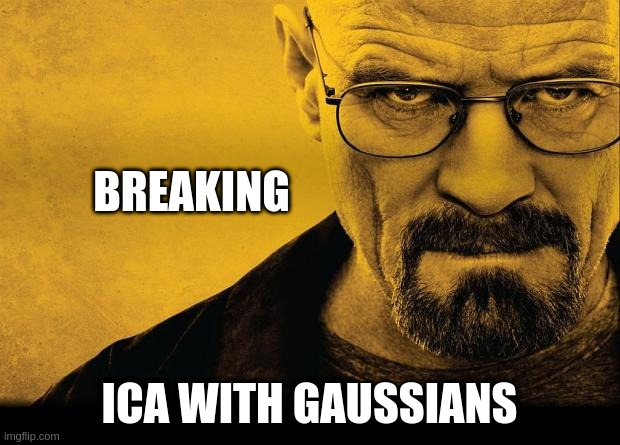
\includegraphics[width=0.4\textwidth]{./img/meme_breakingicabadgaussian}\\
    And \textbf{white}ning won't help either.
    \end{center}
\end{frame}
}

\subsubsection{A formal argument for why Gaussians are bad for ICA}

\begin{frame}{\subsubsecname}

Recall that the joint density of independent sources is a factorizing density:

\begin{equation}
\label{eq:facts}
P_{\vec s}(\vec s) = \prod_{i=1}^{N} P_{s_i}(s_i)  \,.
\end{equation}

If we assumed gaussian distributed sources, the following factorization becomes possible (e.g. $N=2$):

\begin{equation}
	\label{eq:factsgauss}
	\begin{array}{ll}
	P_{\vec{s}}({\vec{s}}) 
	& = \frac{1}{2\pi} 
    \exp \left( -\frac{\lVert{\vec{s}}\rVert^2}{2} \right)
	\\
	& = \underbrace{
	\Bigg[ \frac{1}{\sqrt{2\pi}} \exp \left( -
		\frac{{s_1}^2}{2} \right) \Bigg]
		}_{{P}_{s_1}({s}_1)}
		\underbrace{\Bigg[
			\frac{1}{\sqrt{2\pi}} \exp \left( -
			\frac{{s_2}^2}{2} \right)
		\Bigg]
			}_{{P}_{s_2}({s}_2)}
	\end{array}
\end{equation}
\end{frame}

\begin{frame}{\subsecname~(cont'd)}

%\slidesonly{\textbf{A more formal argument (cont'd):}}

Now consider applying an orthogonal mixing matrix $\widetilde{\vec A}$ that is \textbf{known}. 
\slidesonly{(orthogonal because we whitened the data $\vec x$)\\
Consequently:
}
\notesonly{We've seen how whitening takes an ICA problem with any valid\footnote{invertible} mixing matrix $A$ 
and reformulates it into a new problem with an orthogonal mixing matrix $\widetilde{\vec A}$.
The following holds for such an orthogonal mixing matrix $\widetilde{\vec A}$:
}
\begin{equation}
\widetilde{\vec A}^\top = \widetilde{\vec A}^{-1} \Leftrightarrow \widetilde{\vec A}^{-1}\widetilde{\vec A}=\vec I_N \qquad \text{and} \qquad |\det \widetilde{\vec A}| = |\det \widetilde{\vec A}^\top| = 1
\end{equation}

\begin{equation}
\vec s = \widetilde{\vec A}^{-1} \vec{x} = \widetilde{\vec A}^\top \vec x
\end{equation}

\pause

\notesonly{
We are now interested in the joint density $P_x(\vec x)$ of the mixtures $x_1$ and $x_2$.
}

Density transformation tells us that:
\begin{equation}
	\label{eq:gausstransformeddt}
	{P}_{\vec x}(\vec x) = 
    {P}_{\vec s}(\vec s)  \left|\det \frac{\partial \vec s}{\partial \vec x}\right| 
    = {P}_{\vec s}(\vec s)  \left|\det  \widetilde{\vec A}^{-1}\right|
    = {P}_{\vec s}(\vec s)  \left|\det  \widetilde{\vec A}^\top\right|
\end{equation}
Therefore,
\slidesonly{
\begin{equation}
	{P}_{\vec x}(\vec x)
	= \frac{1}{2\pi} 
    \exp \left( 
    -\frac{\lVert{\widetilde{\vec A}^\top \vec x}\rVert^2}{2} 
    \right)
    \left|\det  \widetilde{\vec A}^\top\right|
	= \ldots?
\end{equation}
}
\end{frame}

\begin{frame}{\subsecname~(cont'd)}
\slidesonly{
Orthogonal mixing matrix $\widetilde{\vec A}$ implies:
$$
\widetilde{\vec A}^\top = \widetilde{\vec A}^{-1} \Leftrightarrow \widetilde{\vec A}^{-1}\widetilde{\vec A}=\vec I_N \qquad \text{and} \qquad |\det \widetilde{\vec A}| = |\det \widetilde{\vec A}^\top| = 1
$$
$$
\vec s = \widetilde{\vec A}^{-1} \vec{x} = \widetilde{\vec A}^\top \vec x
$$}
\begin{align}
    \label{eq:gaussx}
	{P}_{\vec x}(\vec x)
	&= \frac{1}{2\pi} 
    \exp
    \Big(
    -\frac{
    \overbrace{
    \lVert{\widetilde{\vec A}^\top \vec x}\rVert^2
    }^{\mathclap{
		\lVert{\widetilde{\vec A}^\top \vec x}\rVert^2
		= \left(\widetilde{\vec A}^\top \vec x\right)^\top \widetilde{\vec A}^\top \vec x
		\,=\, \vec x^\top \widetilde{\vec A} \, \widetilde{\vec A}^\top \vec x
		= \vec x^\top \vec x
		= \lVert{\vec x}\rVert^2
		}}}{2}
    \Big)
    \underbrace{
    \left|\det  \widetilde{\vec A}^\top\right|
    }_{=\, 1}
    \\
	&= \frac{1}{2\pi} 
    \exp \left( 
    -\frac{\lVert{\vec x}\rVert^2}{2} 
    \right)\\
    \label{eq:gaussxfact}
	& = \underbrace{
	\Bigg[ \frac{1}{\sqrt{2\pi}} \exp \left( -
		\frac{{x_1}^2}{2} \right) \Bigg]
		}_{{P}_{x_1}({x}_1)={P}_{s_1}({s}_1)}
		\underbrace{\Bigg[
			\frac{1}{\sqrt{2\pi}} \exp \left( -
			\frac{{x_2}^2}{2} \right)
		\Bigg]
			}_{{P}_{x_2}({x}_2)={P}_{s_2}({s}_2)}
            \text{no change in pdf!}
\end{align}
\end{frame}

\notesonly{
We see that the factorization in \eqref{eq:gaussxfact} describes the pdf for the mixtures $\vec x$ identically to the pdf of the original sources. 
The original and mixed distributions are identical. The mixing matrix did not change this. Therefore, it would be impossible to find its corresponding unmixing matrix to undo the rotation.
}

\begin{frame}{\subsecname~(cont'd)}

\notesonly{
Mixing two independent Gaussians leads to a joint mixed distribution that is equal to that of the original sources.
This is actually justified by the property that \emph{
uncorrelated jointly Gaussian variables are necessarily independent.}\footnote{
Further details can be found in Hyv{\"a}rinen Ch. 2.5.
}
}

A mixture of sources where, at most, one is Gaussian, can still be separated by ICA. It only becomes a problem when we have more than one Gaussian.


\slidesonly{
\begin{minipage}{0.65\textwidth}

\svspace{5mm}

\begin{itemize}
\item Mixing two independent Gaussians leads to a joint mixed distribution ${P}_{\vec x}(\vec x)$ that is effectively equal to the joint distribution of the original sources ${P}_{\vec s}(\vec s)$.\\

\pause

\item No surprise: \emph{uncorrelated jointly Gaussian variables are necessarily independent.}
\pause

\pause 

\item One Gaussian + other distribution(s) is fine.
\item Two ore more Gaussians. No way.
\end{itemize}
\end{minipage}
}

\slidesonly{
\only<2>{
	\placeimage{10.5}{6}{img/meme_icagaussian}{width=4cm}%
}
\only<4>{
	\placeimage{10.5}{6}{img/meme_nomoregaussians}{width=4cm}%
}
}
\end{frame}
